\documentclass[a4paper,11pt]{article}
\usepackage[utf8]{inputenc}
\usepackage[normalem]{ulem}
\usepackage{graphicx, hyperref, caption, amsmath, amssymb, amsthm, subcaption, tabularx, float, fullpage, url,dsfont, tipa, textcomp, braket, physics, grffile, color,  multicol,wasysym,slantsc, url, color}
\usepackage[dutch]{babel}
\usepackage{graphicx}
\usepackage{listings,caption,subcaption}
\usepackage[margin=2cm]{geometry}
\usepackage[dvipsnames]{xcolor}
%\usepackage{preamble}
\usepackage{enumitem}
\usepackage{gensymb}
\usepackage{circuitikz}
\usetikzlibrary{patterns}
\usetikzlibrary{decorations.pathmorphing,patterns}

\newcommand{\stkout}[1]{\ifmmode\text{\sout{\ensuremath{#1}}}\else\sout{#1}\fi}

%\usepackage{subcaption}
%%%%%%%%%%%%%%%%%%%%%%%%%%%%%%%%%%%%%%%%
\title{Examen AN1}


\begin{document}

\section*{Optie 1: Staafje \& schijf}
\subsection*{Opgave}
Een schijfje met puntmassa $m_1$ en een massieve staaf met lengte $\ell=4d$ en massa $m_2$ liggen op een wrijvingsloze tafel. Het schijfje vliegt met een snelheid $v_0 \hat{j}$ in de $y$-richting tegen de staaf, die in de richting van de $x$-as gepositioneerd is (zie figuur \ref{fig:VoorBotsing}). Als het schijfje de staaf raakt op een afstand $d$ van de midden, dan zal het schijfje verder bewegen met snelheid $\vec{v}_1$ en de staaf met een lineaire snelheid $\vec{v}_2$. Verder zal de staaf ook beginnen roteren (zie figuur \ref{fig:NaBotsing}). De richtingen van $\vec v_1$ en $\vec v_2$ op deze tekeningen zijn willekeurig gekozen. Als je aanneemt dat er behoud van energie is tijdens de botsing toon dan aan dat:
\begin{enumerate}[label=(\alph*)]
	\item $\vec{v}_1$ voldoet aan
	\begin{equation}
		v_0^2=v_{1,x}^2+v_{1,y}^2+\alpha v_{1,x}^2+\alpha(v_0-v_{1,y})^2+3\alpha(v_0-v_{1,y})^2
	\end{equation}
	waar $\alpha=m_1/m_2$.
	\item Toon aan dat gegeven een $v_{1,x}$, er precies twee oplossingen zijn voor $v_{1,y}$ als en slechts als
	\begin{equation}
		v_0^2>(1+4\alpha)(1+\alpha)v_{1,x}^2.
	\end{equation}
	\item Nu gaan we voor de gemakkelijkheid aannemen dat $v_{1,x}=0$. Er zijn nu twee mogelijke oplossingen voor $v_{1,y}$. De eerste is wanneer het schijfje dwars door de staaf gaat en ze elkaar dus niet zouden raken. Wat is de andere oplossing?
\end{enumerate}
\begin{figure}[H]
	\centering
	\begin{subfigure}[b]{0.45\textwidth}
		\centering
		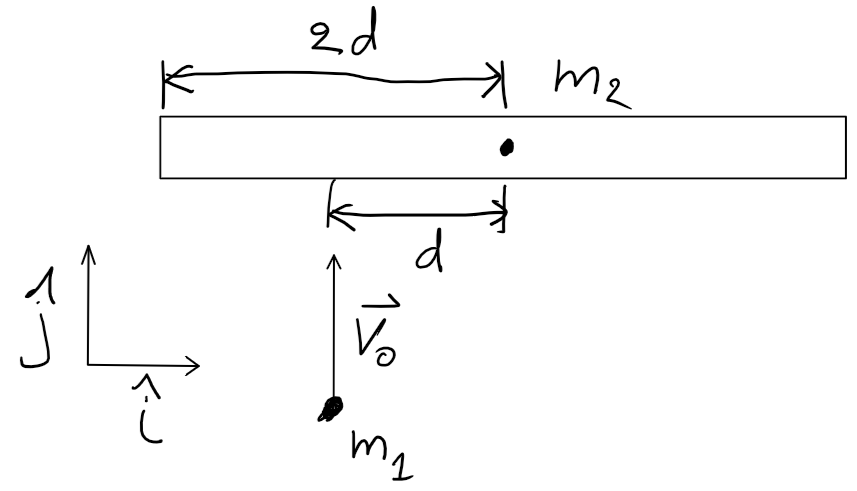
\includegraphics[width=\textwidth]{VoorBotsing}
		\caption{}
		\label{fig:VoorBotsing}
	\end{subfigure}
	\hfill
	\begin{subfigure}[b]{0.45\textwidth}
		\centering
		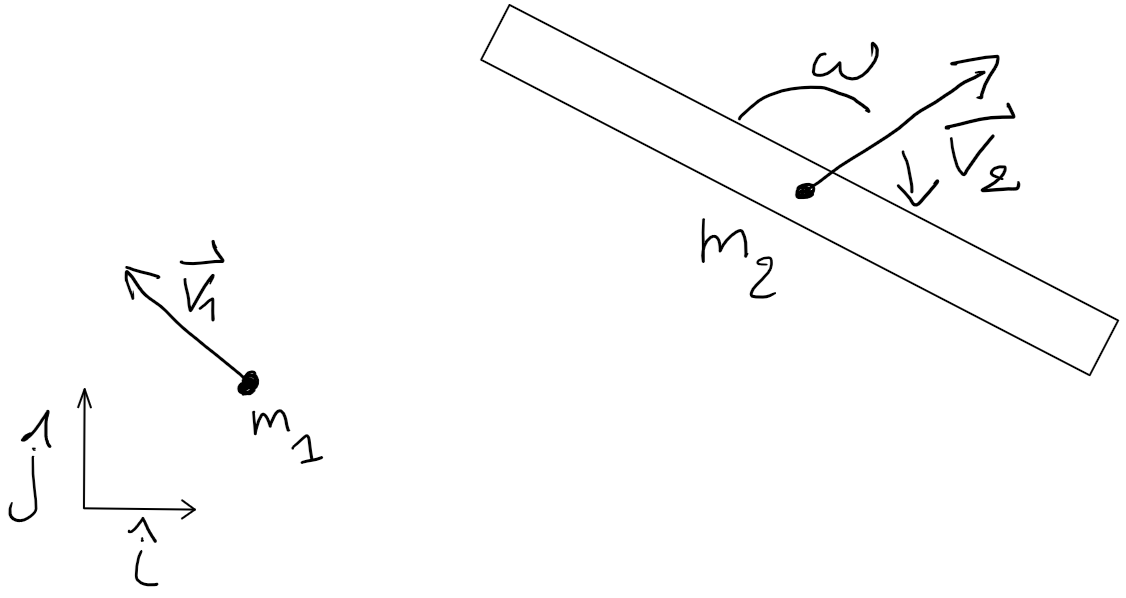
\includegraphics[width=\textwidth]{NaBotsing}
		\caption{}
		\label{fig:NaBotsing}
	\end{subfigure}
	\caption{Figuur \ref{fig:VoorBotsing} geeft de situatie voor de botsing weer en figuur \ref{fig:NaBotsing} die na de botsing.}
	\label{fig:Botsing}
\end{figure}


\newpage 
\section*{Optie 2: Veren en evenwicht}
\subsection*{Opgave}
Een dunne staaf van lengte $L$ en massa $M$ is aan de rechterkant verbonden met het plafond via aan een lineaire veer (veerconstane $k$). Aan de linkerkant is de staaf verbonden met een muur, waarbij een torsieveer (angulaire veerconstante $\kappa$) dienst doet als scharnier. Dit systeem is in evenwicht wanneer de staaf horizontaal is, zoals getekend in figuur \ref{fig:veren}. In dit geval heeft de lineare veer een uitrekking $y_0$ t.o.v. zijn rustlengte, en de torsieveer een uitwijkingshoek $\theta_0$. 
\\ \\
Wanneer de staaf onder een kleine hoek $\theta$ uit de evenwichtspositie gehaald wordt, vindt er een oscillatie plaats bij het loslaten. Leid de frequentie $f$ af van deze oscillatiebeweging als een functie van $M$, $L$, $k$ en $\kappa$.

\subsection*{Extra uitleg}
\begin{itemize}
    \item Het traagheidsmoment van een dunne staaf rond zijn massamiddelpunt is:
\begin{equation}
    I=\frac{1}{12}ML^2.
\end{equation}
    \item  Een torsieveer (figuur \ref{fig:torsieveer}) is het angulair equivalent van de gekende, lineaire veer. Dit type veer veroorzaakt een krachtmoment $\tau$ volgens de angulaire wet van Hooke:
    \begin{equation}
       \tau = -\kappa \theta,
    \end{equation}
    waarbij $\kappa$ de angulaire veerconstante is met eenheden ${\rm N\, m/rad }$ en $\theta$ de openingshoek t.o.v. de rusthoek.
    \end{itemize}

\begin{figure}[H]
    \centering
    \begin{subfigure}{0.45\textwidth}
        \begin{circuitikz}
        
        % Vertical wall
        \fill[pattern=north east lines] (0,3) rectangle (0.25,5);
        \draw (0.25,3) -- (0.25,5);
        
         % Horizontal wall
        \fill[pattern=north east lines] (3.5,7.75) rectangle (4.5,8);
        \draw (3.5,7.75) -- (4.5,7.75);
        
        % Torsion spring & rod
        \node[circle,draw] (c) at (0.425,3.965){};
        \node at (0.55,3.65){$\kappa$};
        \draw[fill=gray!35] (0.6,4.02) rectangle (4,3.92) node[midway,above]{$M$} ;
        
        % Regular spring
        \draw[decoration={aspect=0.7, segment length=3mm, amplitude=1.2mm,pre length = 1mm, post length =0.3mm,coil},decorate](4,7.75) -- (4,4) node[midway, right]{$k$};
        
        % Connection points
        \filldraw (4,3.98) circle (1pt);
        \filldraw (4,7.75) circle (1pt);
        
        % Measurements
        \draw[<->] (0.6,3.3) -- (4,3.3) node[midway, below] {$L$};
        \draw[|->] (4.75,5) -- (4.75,4) node[midway,right] {$y_0$};
        
        \draw (0.55,4.15) -- (1.1,4.7);
        \draw[<-] (1.1,4.1) arc [start angle=0, end angle=45, x radius=0.5, y radius=0.5] node[midway,right] {$\theta_0$};
        
        \end{circuitikz}
    \caption{Opstelling}
    \label{fig:veren}
    \end{subfigure}
    \begin{subfigure}{0.45\textwidth}
        \centering
        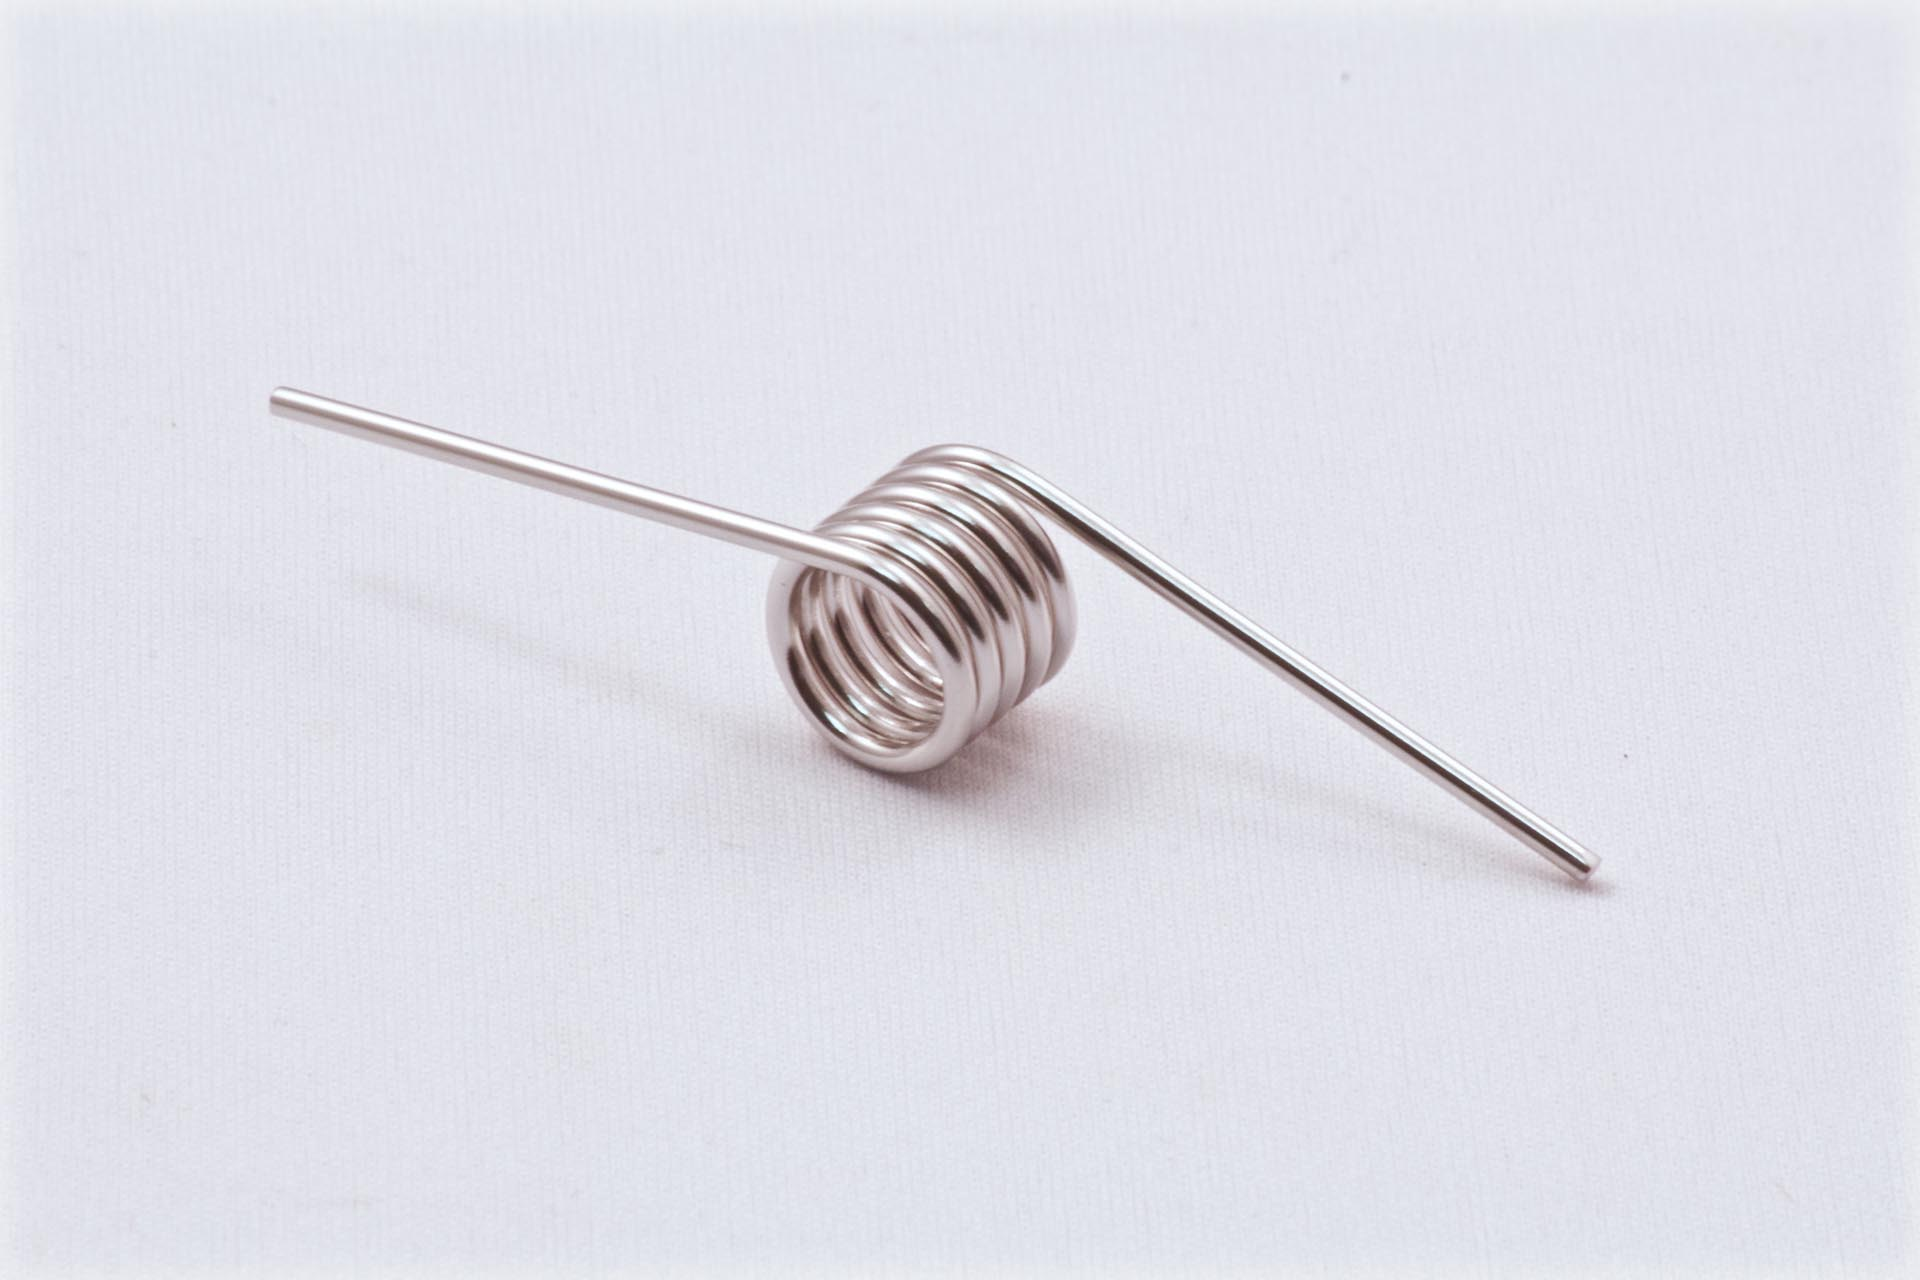
\includegraphics[width=0.45\textwidth]{torsion_spring.jpg}
        \caption{Torsieveer}
        \label{fig:torsieveer}
    \end{subfigure}
    \caption{Vraag over veren \& oscillatie}
\end{figure}



\newpage 
\section*{Optie 3: James Bond in de achtervolging}
\subsection*{Opgave}
James Bond is in een achtervolging met een schurk. Beide rijden aan een constante snelheid $v$ over een vlak wegdek. Op een gegeven moment staat er een helling met hoek $\theta$ op hun pad (zie figuur \ref{fig:Bond},a). De helling heeft een hoogte $h_0$. De massa van James Bond en zijn Astin Martin is $M$ en die van de schurk en zijn vluchtwagen is $2M$. Beschouw beide auto's als puntmassa's. Gedurende de hele oefening mag wrijving verwaarloosd worden.
\begin{enumerate}[label=(\alph*)]
    \item De schurk rijdt over de helling en maakt een parabolische beweging (zie figuur \ref{fig:Bond}.b). Wat is het hoogste punt dat de schurk bereikt? Geef $x$- en $y$-coördinaten van dit punt op zijn traject. Veronderstel dat de snelheid van de schurk constant blijft terwijl hij de helling op rijdt.
    \item Op zijn hoogste punt vuurt de schurk een kogel af met massa $m$ onder een hoek $\theta$, zoals getekend in figuur \ref{fig:Bond}.c. Op dat moment rijdt ook James Bond op de helling. Met welke snelheid moet de kogel afgevuurd worden zodat James Bond geraakt wordt? Veronderstel dat de snelheid van James Bond constant blijft terwijl hij de helling op rijdt.
    \item Stel nu dat de schurk nog kon stoppen voor hij de helling op rijdt. James Bond kon echter niet op tijd stoppen en botst met een snelheid $v$ tegen de auto van de schurk. De botsing verloopt volledig elastisch. Bereken de snelheden van James Bond en de schurk net na de botsing. 
\end{enumerate}

\begin{figure}[H]
    \centering
    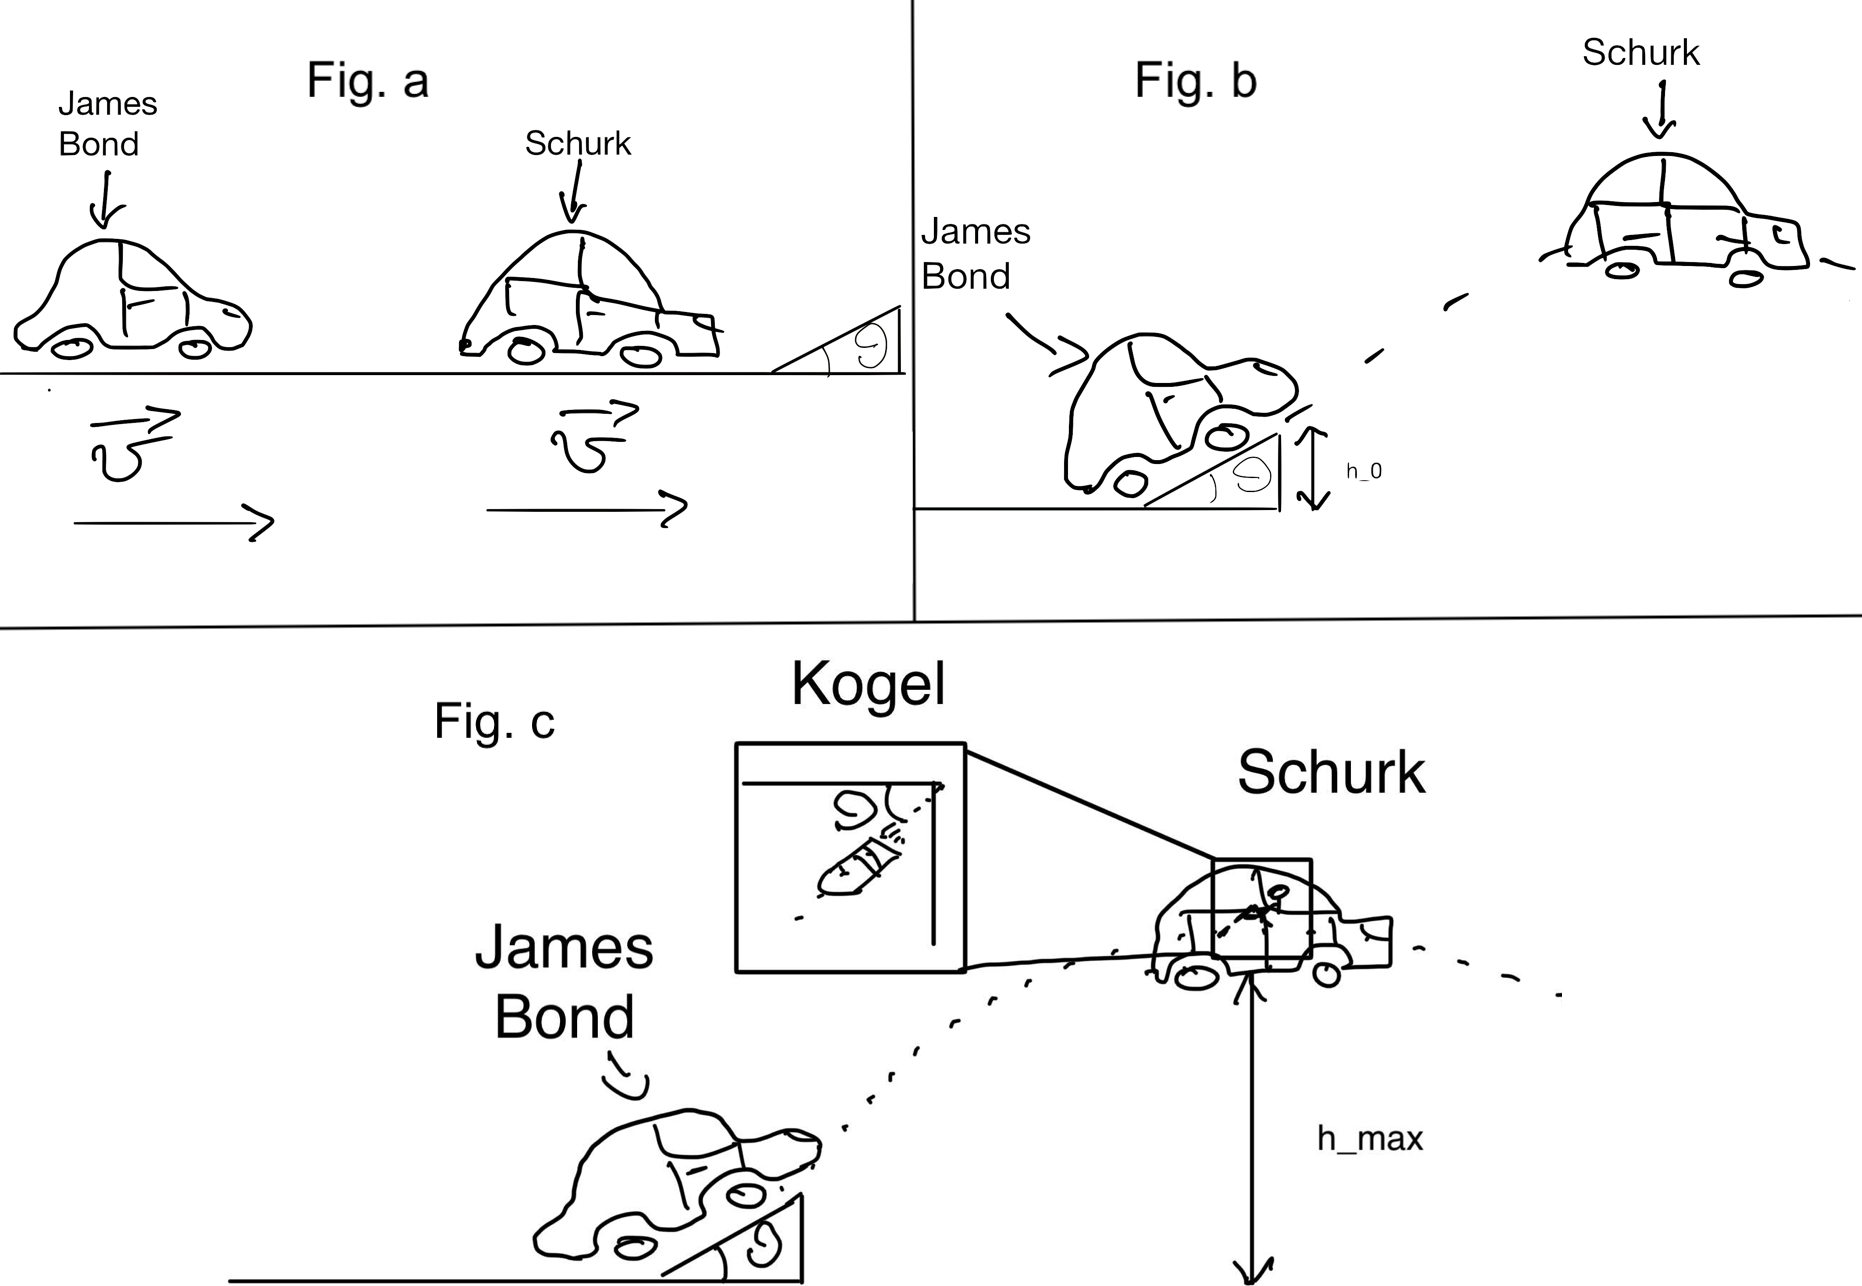
\includegraphics[width = \textwidth]{James_Bond.png} 
    \caption{}
    \label{fig:Bond}
\end{figure}



\newpage
\section*{Optie 4: Traagheidsmomenten \& energie}
\subsection*{Opgave}
Er worden drie objecten met constante massadichtheid $\sigma$ geroteerd met hoeksnelheid $\omega$ rondom een punt $P$. De eerste is een massieve schijf met als middelpunt $P$ en als straal $R$ (zie figuur \ref{fig:Schijf1}). De tweede is een massieve schijf met straal $R/2$ die rechts van het punt $P$ ligt (zie figuur \ref{fig:Schijf2}). De derde schijf is schijf 1, waar schijf 2 uit weggehaald werd (zie figuur \ref{fig:Schijf3}).
\begin{enumerate}[label=(\alph*)]
	\item Toon aan wat de traagheidsmomenten $I_1,I_2$ en $I_3$ zijn van de eerste, tweede en derde schijf respectievelijk.
	\item Toon aan dat de kinetische energie van de rotatie van schijf 1 gelijk is aan de som van kinetische energie\"en van de andere twee schijven.
\end{enumerate}
\begin{figure}[H]
	\centering
	\begin{subfigure}[b]{0.25\textwidth}
		\centering
		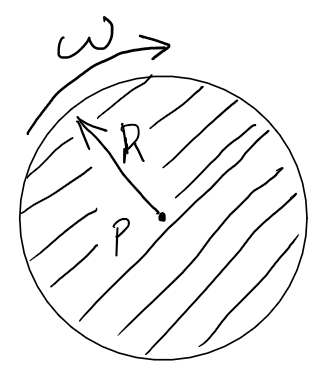
\includegraphics[width=\textwidth]{Schijf1}
		\caption{}
		\label{fig:Schijf1}
	\end{subfigure}
	\hfill
	\begin{subfigure}[b]{0.25\textwidth}
		\centering
		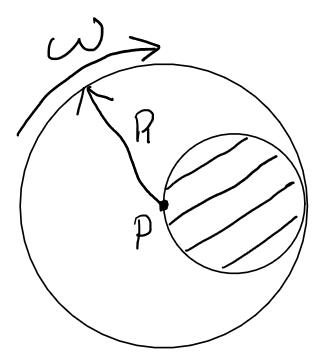
\includegraphics[width=\textwidth]{Schijf2}
		\caption{}
		\label{fig:Schijf2}
	\end{subfigure}
	\hfill
	\begin{subfigure}[b]{0.25\textwidth}
		\centering
		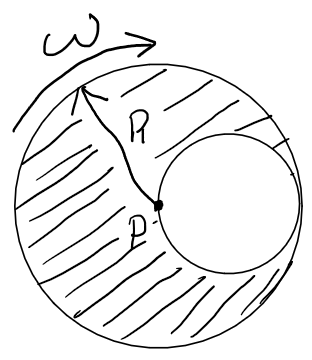
\includegraphics[width=\textwidth]{Schijf3}
		\caption{}
		\label{fig:Schijf3}
	\end{subfigure}
	\caption{Dit zijn drie verschillende objecten (gearceerde delen) die met hoeksnelheid $\omega$ geroteerd worden rondom punt $P$.}
	\label{fig:Schijven}
\end{figure}



\end{document}